\documentclass[italian,a4paper]{article}
\usepackage[tight,nice]{units}
\usepackage{babel,amsmath,amssymb,amsthm,graphicx,url}
\usepackage[text={5.5in,9in},centering]{geometry}
\usepackage[utf8x]{inputenc}
\usepackage[T1]{fontenc}
\usepackage{ae,aecompl}
\usepackage[footnotesize,bf]{caption}
\usepackage[usenames]{color}
\usepackage{textcomp}
\usepackage{gensymb}
%\include{pstricks}
\frenchspacing
\pagestyle{plain}
%------------- eliminare prime e ultime linee isolate
\clubpenalty=9999%
\widowpenalty=9999
%--- definizione numerazioni
\renewcommand{\theequation}{\thesection.\arabic{equation}}
\renewcommand{\thefigure}{\arabic{figure}}
\renewcommand{\thetable}{\arabic{table}}
\addto\captionsitalian{%
  \renewcommand{\figurename}%
{Grafico}%
}
%
%------------- ridefinizione simbolo per elenchi puntati: en dash
%\renewcommand{\labelitemi}{\textbf{--}}
\renewcommand{\labelenumi}{\textbf{\arabic{enumi}.}}
\setlength{\abovecaptionskip}{\baselineskip}   % 0.5cm as an example
\setlength{\floatsep}{2\baselineskip}
\setlength{\belowcaptionskip}{\baselineskip}   % 0.5cm as an example
%--------- comandi insiemi numeri complessi, naturali, reali e altre abbreviazioni
\renewcommand{\leq}{\leqslant}
%--------- porzione dedicata ai float in una pagina:
\renewcommand{\textfraction}{0.05}
\renewcommand{\topfraction}{0.95}
\renewcommand{\bottomfraction}{0.95}
\renewcommand{\floatpagefraction}{0.35}
\setcounter{totalnumber}{5}
%---------
%
%---------
\begin{document}
\title{Relazione di laboratorio: effetto Faraday}
\author{\normalsize Ilaria Brivio (582116)\\%
\normalsize \url{brivio.ilaria@tiscali.it}%
\and %
\normalsize Matteo Abis (584206)\\ %
\normalsize \url{webmaster@latinblog.org}}
\date{\today}
\maketitle
%------------------
\section{Obiettivo dell'esperienza}
Con questa esperienza si vuole analizzare la rotazione del piano di polarizzazione di un fascio luminoso dovuta al passaggio attraverso un materiale diamagnetico immerso in un campo magnetico esterno, per verificare la validità della legge di Faraday e ricavare una stima della costante di Verdet.
\section{Descrizione dell'apparato strumentale}
L'apparato è composto da una serie di elementi montati su un banco ottico: davanti a una sorgente luminosa sono posizionati un filtro giallo per avere luce monocromatica di lunghezza d'onda $\lambda$=\unit[5893]{\AA{}}, un doppietto di Dollond che renda il fascio parallelo e un polaroid che lo polarizzi linearmente.
La luce passa quindi attraverso un cilindro di vetro di lunghezza $l_v=\unit[11.0]{cm}$ avvolto in una bobina di $N= 3660$ spire e lunga $l_b=\unit[18.0]{cm}$. Tale bobina è collegata a un generatore di corrente di intensità regolabile che permette di variare il campo magnetico applicato.

Oltre il cilindro è presente un analizzatore, ovvero un polaroid montato su una ghiera che può compiere una rotazione completa ed è azionata in modo automatico.
All'estremità dell'apparato si trova infine un rivelatore di intensità luminosa. 

L'acquisizione dei dati avviene attraverso un programma che gestisce i movimenti dell'analizzatore e raccoglie le misure del fotodiodo in corrispondenza della posizione angolare della ghiera.
\section{Descrizione della metodologia di misura}
Le misure sono state effettuate una prima volta senza applicare alcun campo magnetico, registrando i valori di intensità del segnale luminoso durante una rotazione completa dell'analizzatore.

La stessa operazione è stata ripetuta facendo passare nella bobina corrente elettrica di intensità pari a 1, 2 e \unit[3]{A}.
\section{Risultati sperimentali ed elaborazione dati}
Dalla legge di Malus, l'intensità della luce trasmessa dall'analizzatore in funzione dell'angolo $\theta$ tra l'asse del polaroid e il piano di polarizzazione segue l'andamento
\begin{equation*}
I(\theta)=\dfrac{I_0}{2}\cos^2\theta 
\end{equation*}

Nei grafici \ref{0amp}, \ref{1amp}, \ref{2amp}, \ref{3amp} sono stati riportati i valori registrati per $I$ al variare dell'angolo di rotazione $\phi$ del polaroid, rispettivamente a circuito aperto e con corrente di intensità 1, 2 e \unit[3]{A}.

L'angolo tra il piano di polarizzazione della luce e l'asse corrispondente alla posizione di zero del polaroid sarà dunque lo sfasamento $\Delta\phi$ della curva trovata rispetto alla funzione $\cos^2\theta$. Per poterlo individuare con maggior precisione è stato eseguita un'interpolazione a due parametri con una funzione del tipo $y=a\cos^2(x+\Delta\phi)$ su due tratti di curva attorno ai due massimi ed è stato estrapolato un valore di $\Delta\phi$ per ciascun fit. Sono state escluse le zone di minimo poiché le misure vicine allo zero sono soggette a un forte errore sistematico dovuto alla sensibilità dello strumento, che risulta evidente dall'appiattimento della curva.

La legge di Faraday lega la rotazione $\Delta\phi$ del piano di polarizzazione all'intensità del campo magnetico in cui è immerso il dielettrico. Nel nostro caso:
\begin{equation*}
\Delta\phi=VBl_v=V\dfrac{\mu_0NI}{l_b}l_v
\end{equation*}
dove $V$ è la costante di Verdet, che dipende in generale dalle caratteristiche del materiale impiegato.

Per poterla verificare sono stati riportati in grafico i due valori trovati per lo sfasamento $\Delta\phi$ in funzione dell'intensità di corrente (Grafico \ref{lin}) ed è stato effettuato un fit lineare sui vari punti.
Dal valore $m$ del coefficiente angolare della retta interpolante si è
infine ricavata la costante di Verdet.
Purtroppo la determinazione della costante
dipende molto dalla regione della curva che si interpola (primo o secondo
massimo) ed è comunque molto lontana dal valore atteso di circa
$\unit[1000]{^\circ / Tm}$. La tabella seguente mostra i risultati ottenuti.
\begin{table}[h]
    \centering
    \begin{tabular}{rl}
        intervallo interpolazione ($^\circ$) & costante di Verdet
        ($\unit[]{^\circ /Tm}$)\\
        1--50 & 1202\\
        1--100 & 1196\\
        180--260 & 1120\\
        130--260 & 1131\\
    \end{tabular}
    \caption{Dati ottenuti per la costante di Verdet.}
    \label{tab:verdet}
\end{table}
Si nota che l'interpolazione non è tanto sensibile
alla porzione di curva scelta, purch\'e si rimanga intorno allo stesso
massimo.
Ulteriori informazioni si possono ricavare dai grafici dei residui relativi
a queste interpolazioni, riportiamo solo quelli relativi alle fasce 1--100 e
130--260, gli altri sono del tutto analoghi. Ogni gruppo di grafici
comprende i dati sulle quattro intensità di corrente da 0 a
\unit[3]{A}.

\begin{figure}[h]
    \begin{center}
        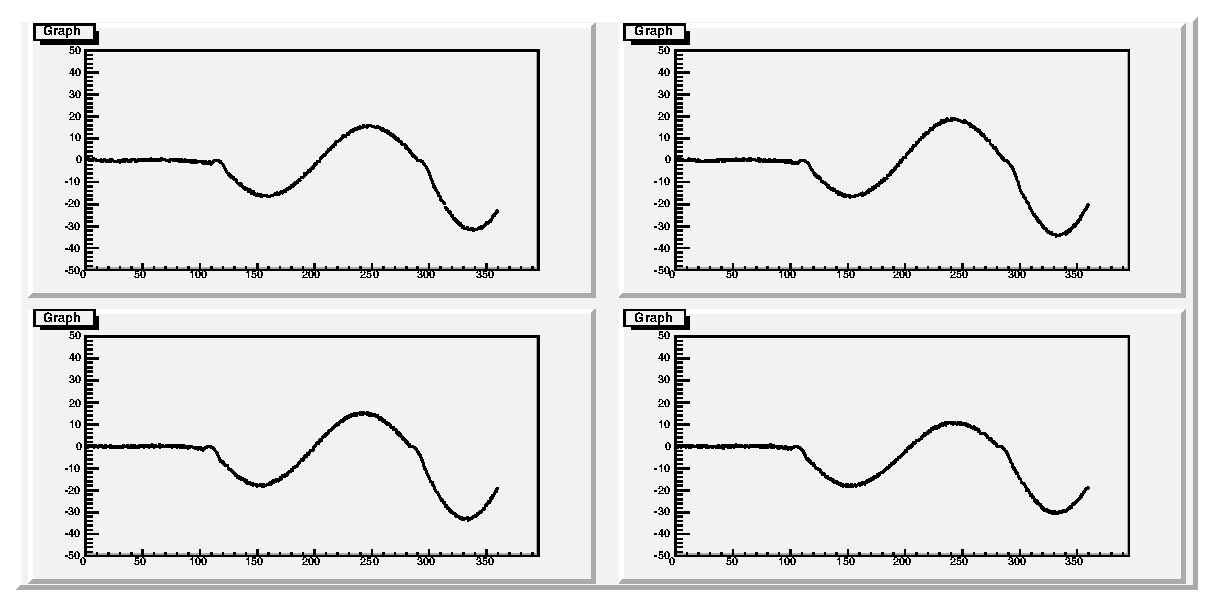
\includegraphics[height=0.4\textheight, width=.9\textwidth]{grafici/1-100r.eps}
    \end{center}
    \caption{Grafico dei residui per l'interpolazione fra 1 e
    $\unit[100]{^\circ}$}
    \label{fig:1100r}
\end{figure}
\begin{figure}[h]
    \begin{center}
        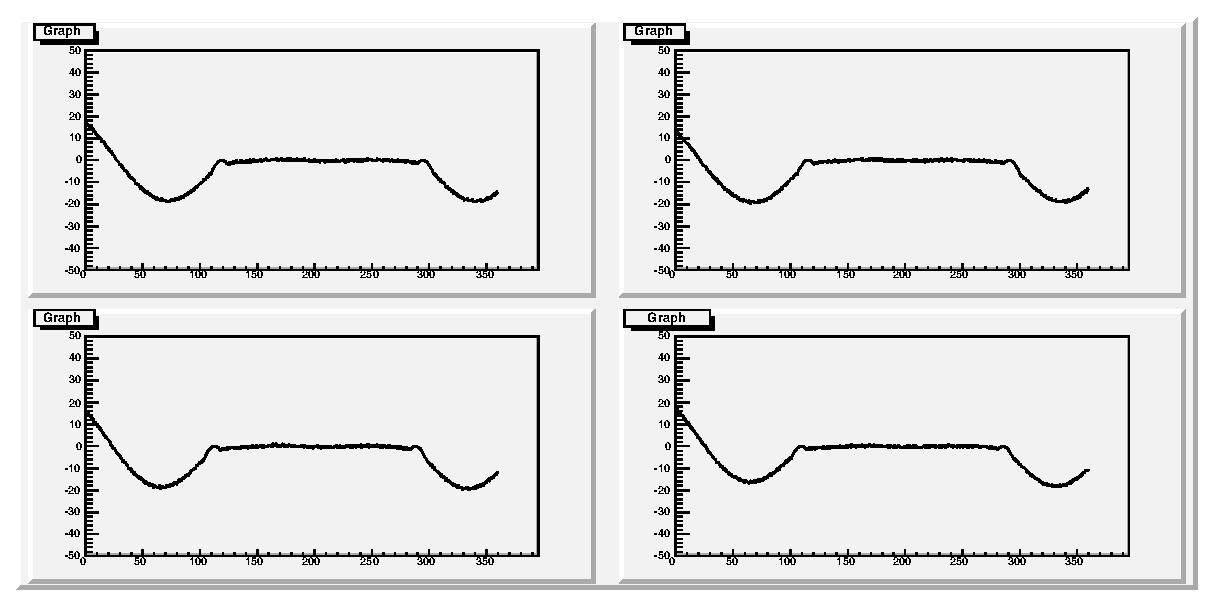
\includegraphics[height=0.4\textheight, width=.9\textwidth]{grafici/130-260r.eps}
    \end{center}
    \caption{Grafico dei residui per l'interpolazione fra 130 e
    \unit[260]{$^\circ$}}
    \label{fig:130260r}
\end{figure}

Dai grafici~\ref{fig:1100r} e~\ref{fig:130260r} \`e evidente come i parametri interpolati per la curva in un massimo siano
completamente inadeguati per quella che dovrebbe essere la stessa curva
nell'altro massimo.

Inoltre i residui presentano una certa struttura fine, anche nel tratto che
con quella scala appare piano. Li riporto nei grafici~\ref{fig:1100rbig}
e~\ref{fig:130260rbig}. Compare in tutti una sequenza a ``M'', indipendente
dall'intensità di corrente.

Tuttavia non è facile ipotizzare a cosa siano dovuti questi strani fenomeni,
non conoscendo nel dettaglio le caratteristiche di molti elementi
delicati dell'apparato strumentale, tra cui certamente possiamo
contare il fotodiodo, l'amplificatore lineare del segnale, il motore che
ruota il polaroid, l'elettronica che controlla il motore stesso e che
comunica con il computer.

In ogni caso ci sembra che da questa analisi altro non si possa
concludere se non che la costante di Verdet del campione utilizzato è tra
1100 e \unit[1200]{$^\circ$/Tm}. Si può stimare il valore come una media con
errore la semidispersione, quindi circa
\begin{equation*}
    V = \unit[1160\pm40]{^\circ/Tm}
\end{equation*}

Per completezza, riporto nei grafici finali anche quelli delle
interpolazioni sulle curve sinusoidali e dell'interpolazione lineare finale.
\begin{figure}[h]
    \begin{center}
        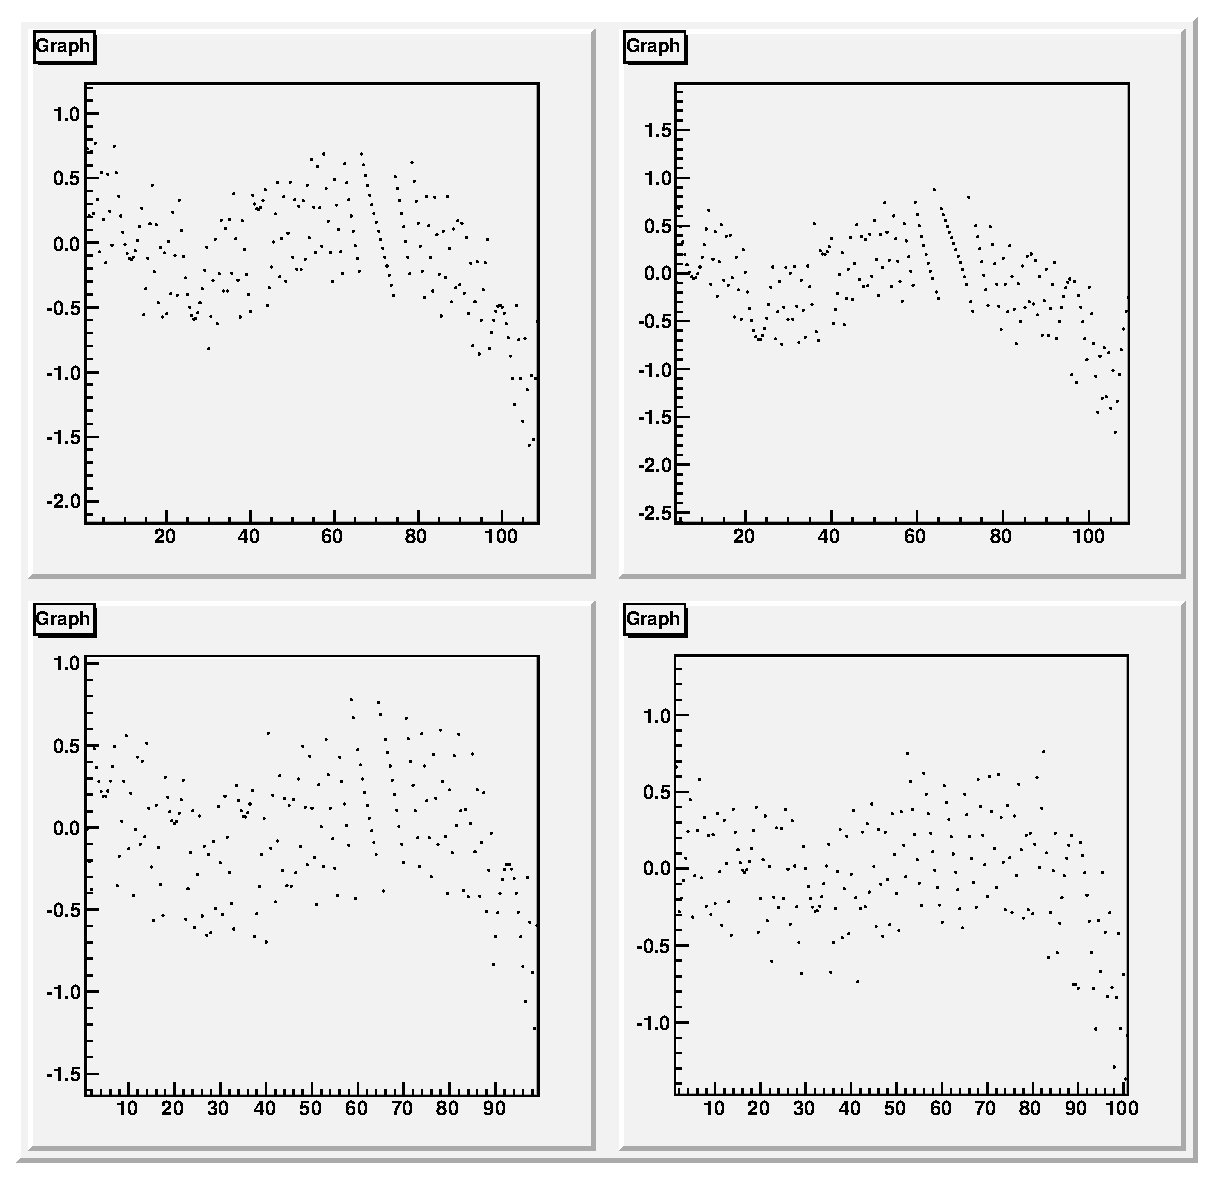
\includegraphics[height=0.4\textheight, width=.9\textwidth]{grafici/1-100r.big.eps}
    \end{center}
    \caption{Grafico dei residui 1-100$^\circ$, ingrandimento.}
    \label{fig:1100rbig}
\end{figure}

\begin{figure}[h]
    \begin{center}
        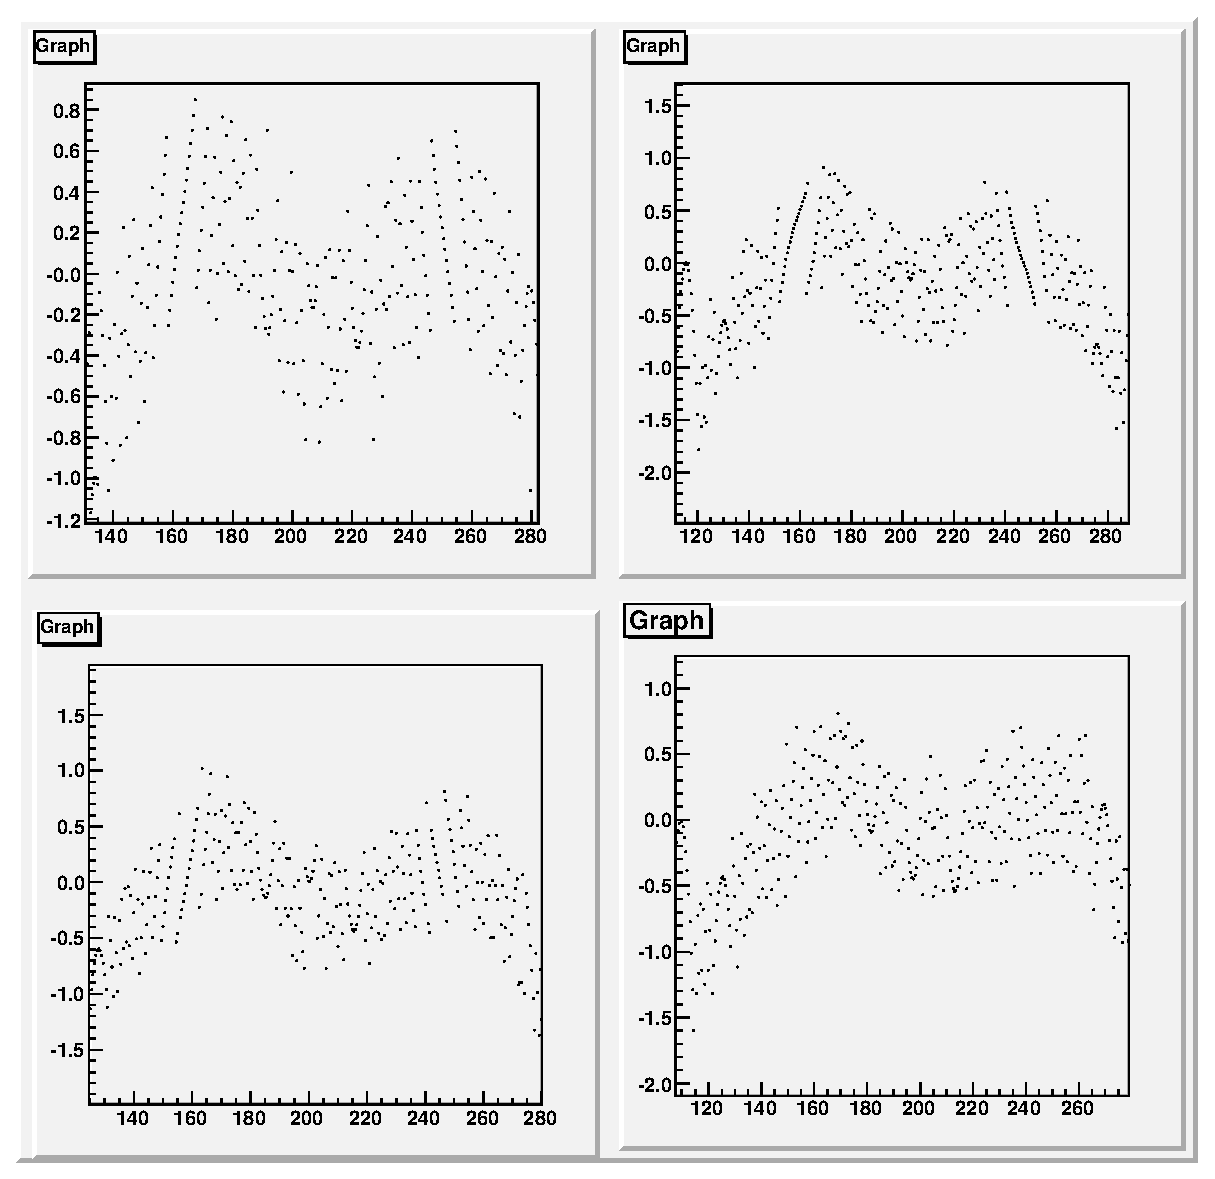
\includegraphics[height=0.4\textheight, width=.9\textwidth]{grafici/130-260r.big.eps}
    \end{center}
    \caption{Grafico dei residui 130-260$^\circ$, ingrandimento.}
    \label{fig:130260rbig}
\end{figure}

\begin{figure}[h]
    \begin{center}
        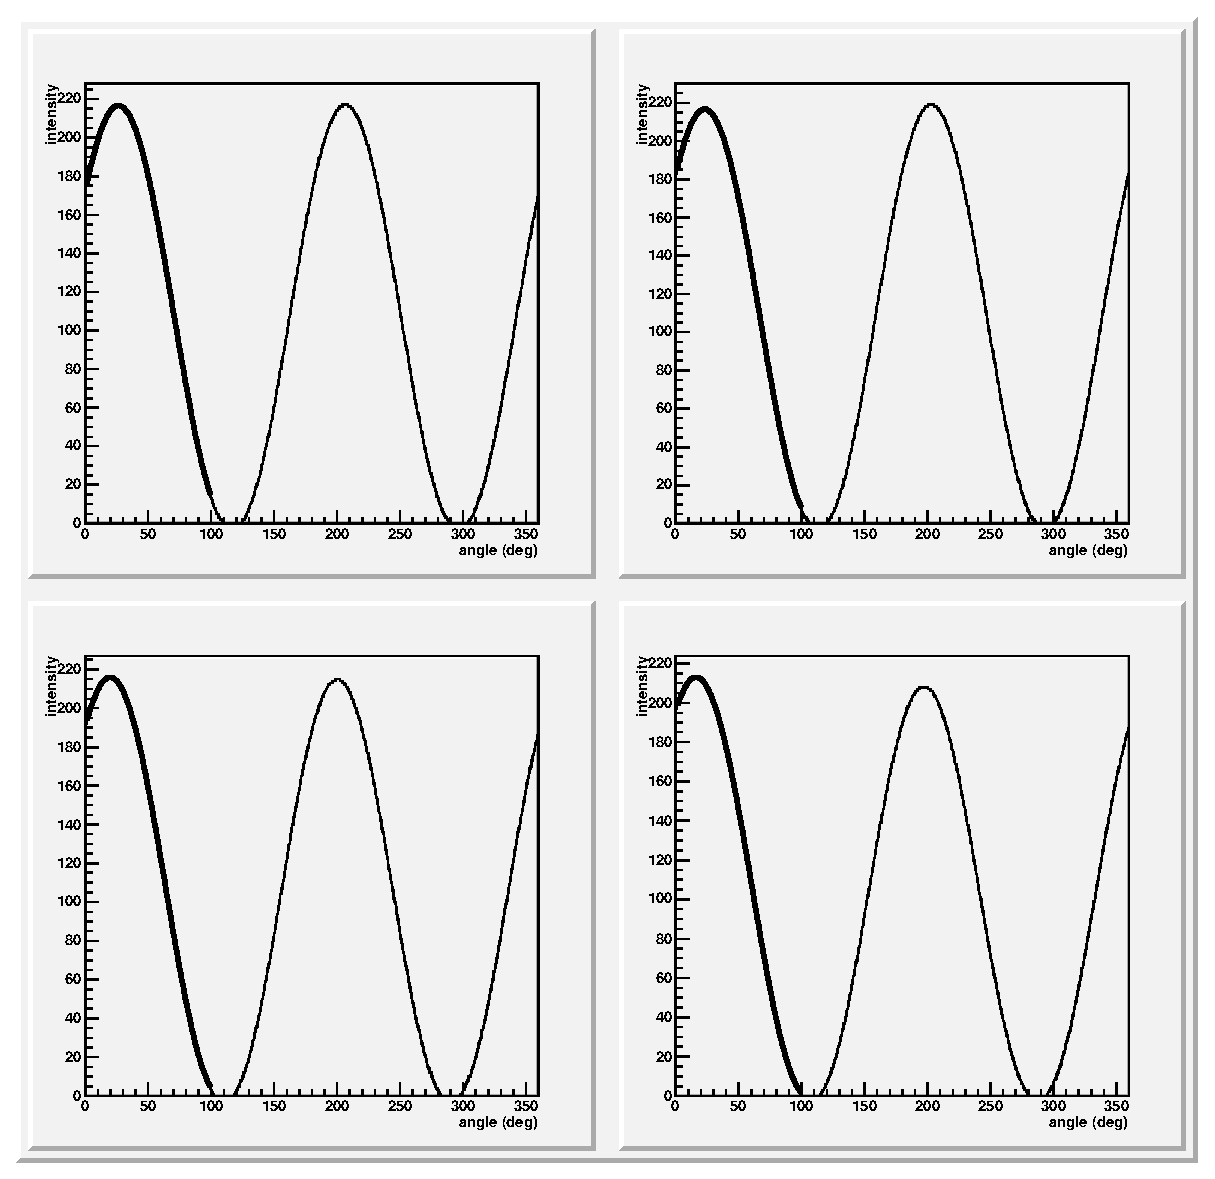
\includegraphics[height=0.4\textheight, width=.9\textwidth]{grafici/1-100g.eps}
    \end{center}
    \caption{Grafico dell'interpolazione 1-100$^\circ$.}
    \label{fig:1100g}
\end{figure}
\begin{figure}[h]
    \begin{center}
        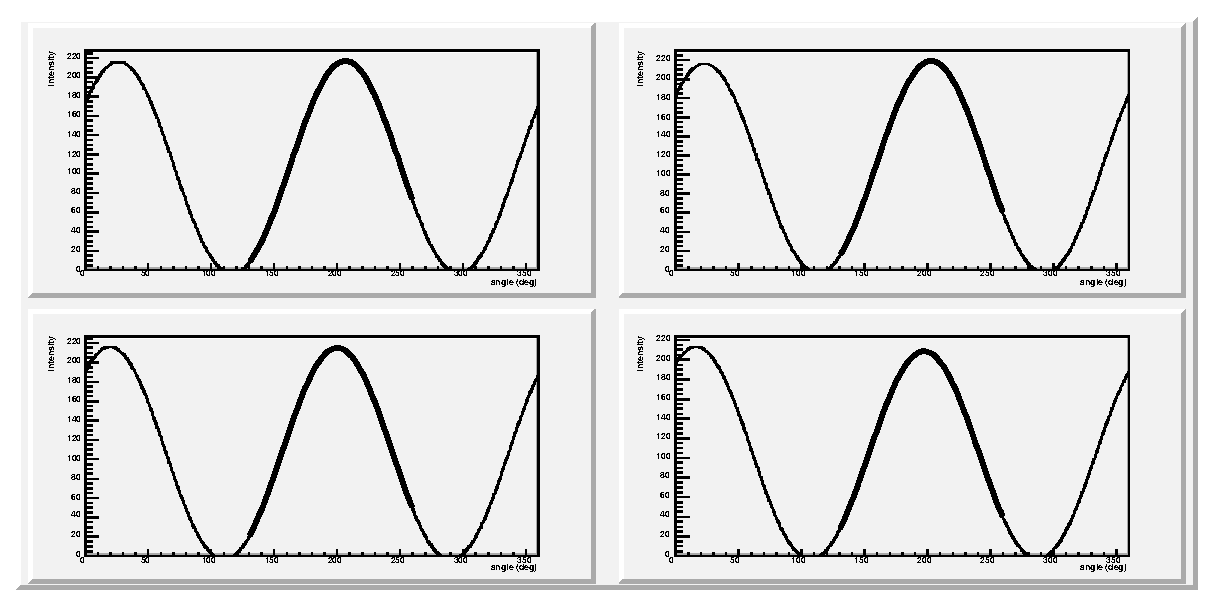
\includegraphics[height=0.4\textheight, width=.9\textwidth]{grafici/130-260g.eps}
    \end{center}
    \caption{Grafico dell'interpolazione 130-260$^\circ$.}
    \label{fig:130260g}
\end{figure}
\begin{figure}[h]
    \begin{center}
        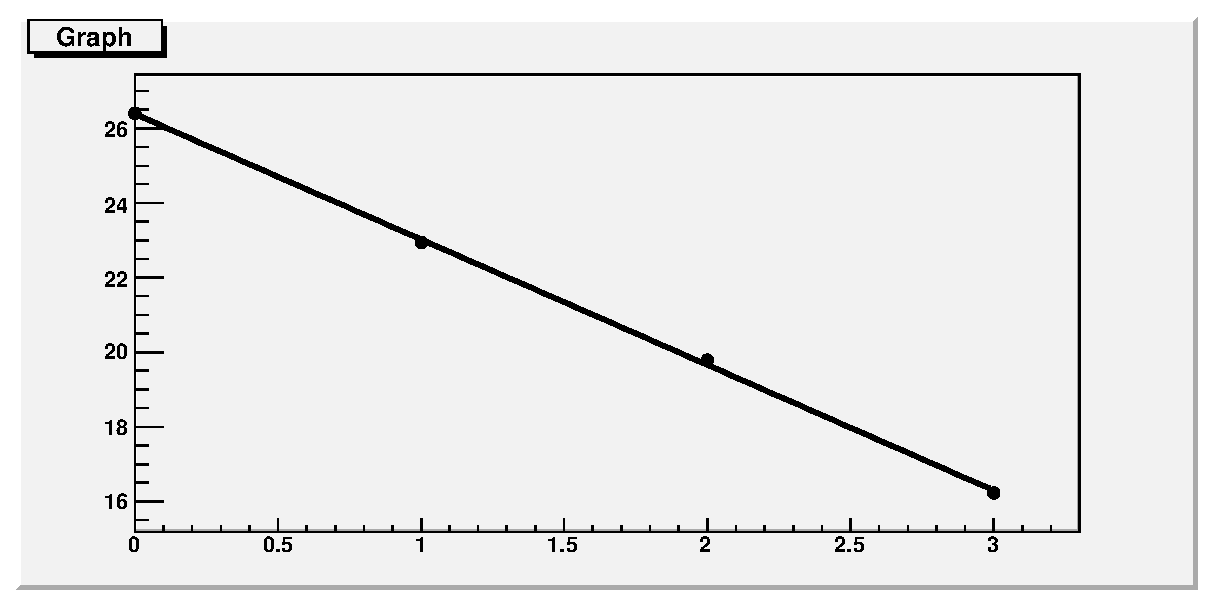
\includegraphics[height=0.4\textheight, width=.9\textwidth]{grafici/1-100verdet.eps}
    \end{center}
    \caption{Grafico dell'interpolazione lineare sui massimi alle quattro
    intensità di corrente, sempre su 1-100$^\circ$.}
    \label{fig:1100g}
\end{figure}
\begin{figure}[h]
    \begin{center}
        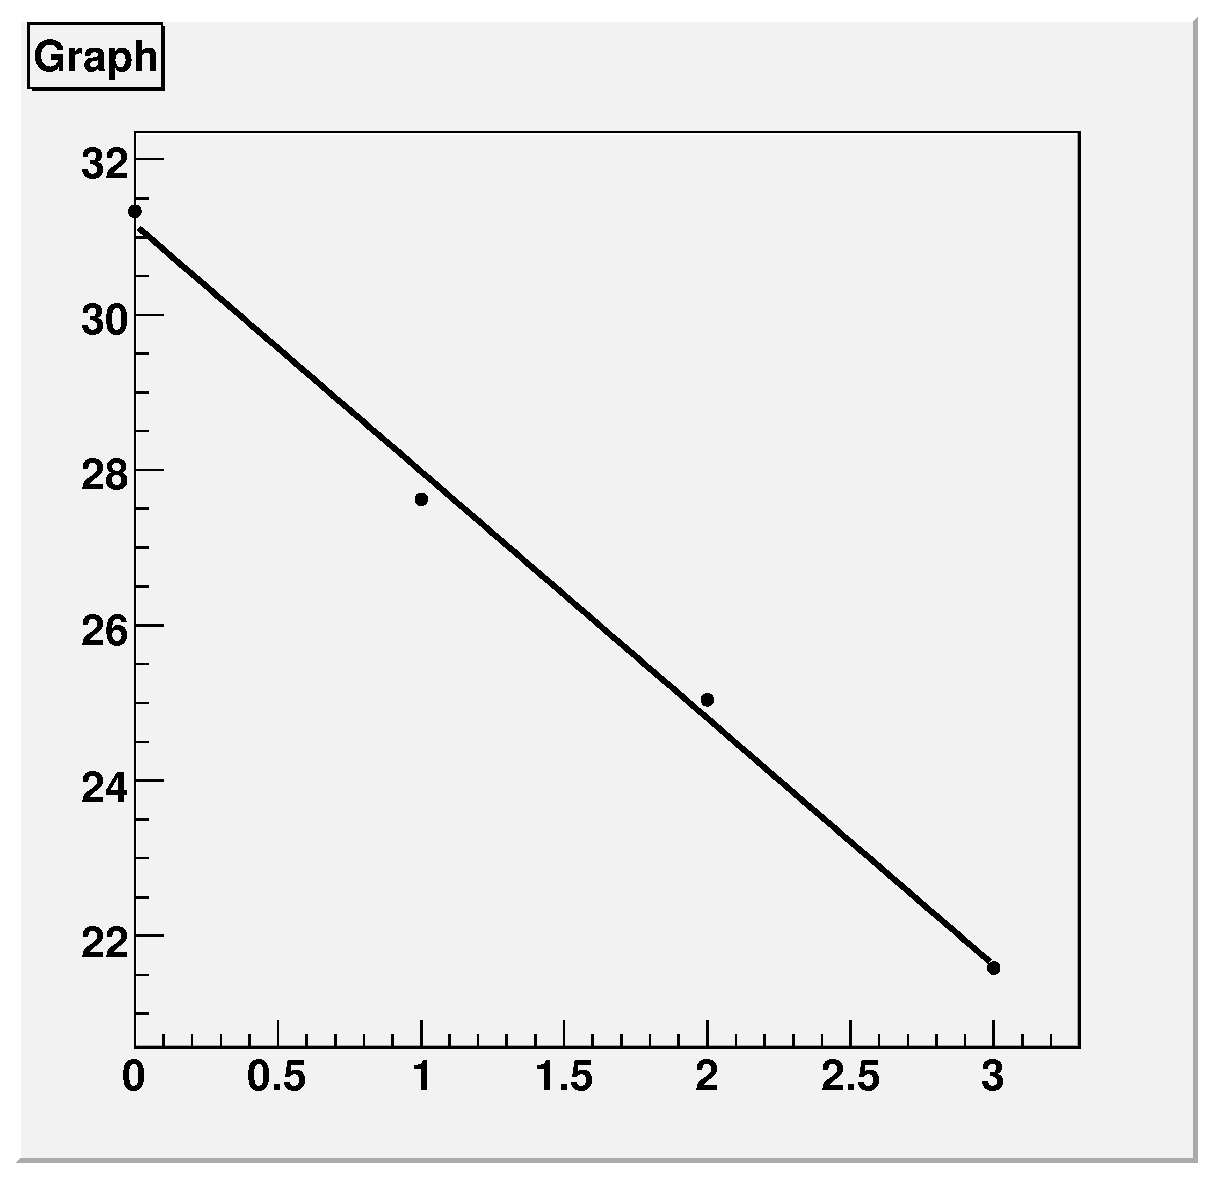
\includegraphics[height=0.4\textheight, width=.9\textwidth]{grafici/130-260verdet.eps}
    \end{center}
    \caption{Grafico dell'interpolazione lineare sui massimi alle quattro
    intensità di corrente, sempre su 130-260$^\circ$.}
    \label{fig:130260g}
\end{figure}
% \section{Conclusioni}

\newpage
\section{Appendice}
\subsection*{Grafici}
\begin{figure}[!h]\centering
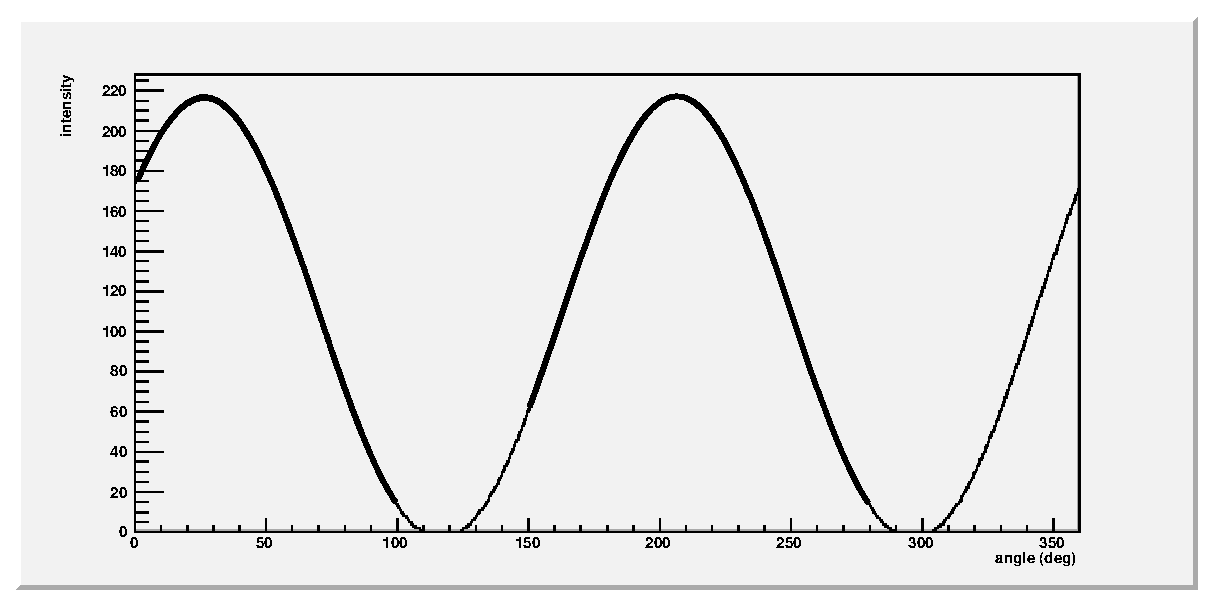
\includegraphics[scale=.6]{0polar.eps}
\caption{Grafico con angolo di rotazione in ascissa e intensità luminosa in ordinata, realizzato in assenza di corrente e dunque di campo magnetico esterno agente sul dielettrico. Attorno ai due massimi sono visibili le curve prodotte dai fit sinusoidali.}\label{0amp}
\end{figure}
\begin{figure}[!h]\centering
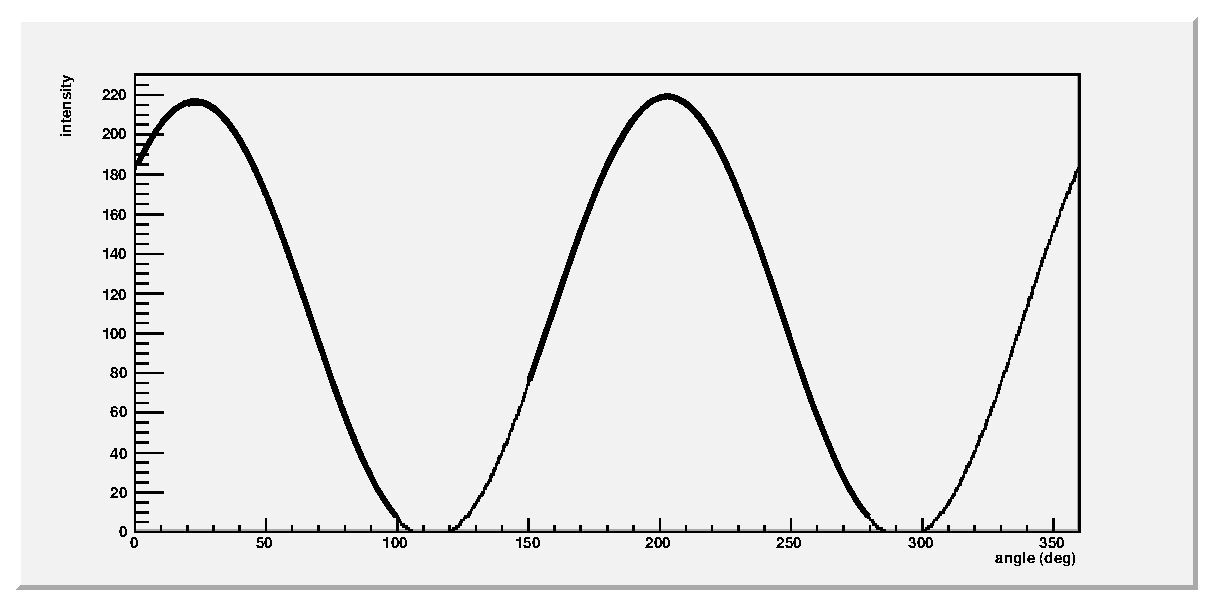
\includegraphics[scale=.6]{1polar.eps}
\caption{Grafico con angolo di rotazione in ascissa e intensità luminosa in ordinata, realizzato con corrente di intensità \unit[1]{A}. Attorno ai due massimi sono visibili le curve prodotte dai fit sinusoidali.}.\label{1amp}
\end{figure}
\begin{figure}[!h]\centering
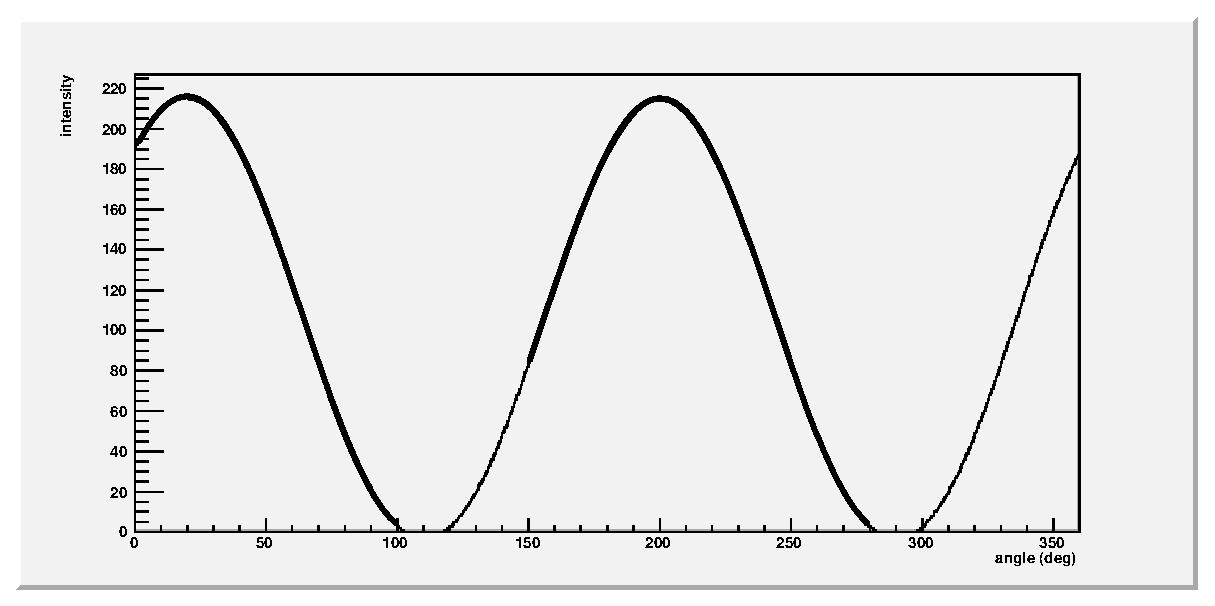
\includegraphics[scale=.6]{2polar.eps}
\caption{Grafico con angolo di rotazione in ascissa e intensità luminosa in ordinata, realizzato con corrente di intensità \unit[2]{A}. Attorno ai due massimi sono visibili le curve prodotte dai fit sinusoidali.}\label{2amp}
\end{figure}
\begin{figure}[!h]\centering
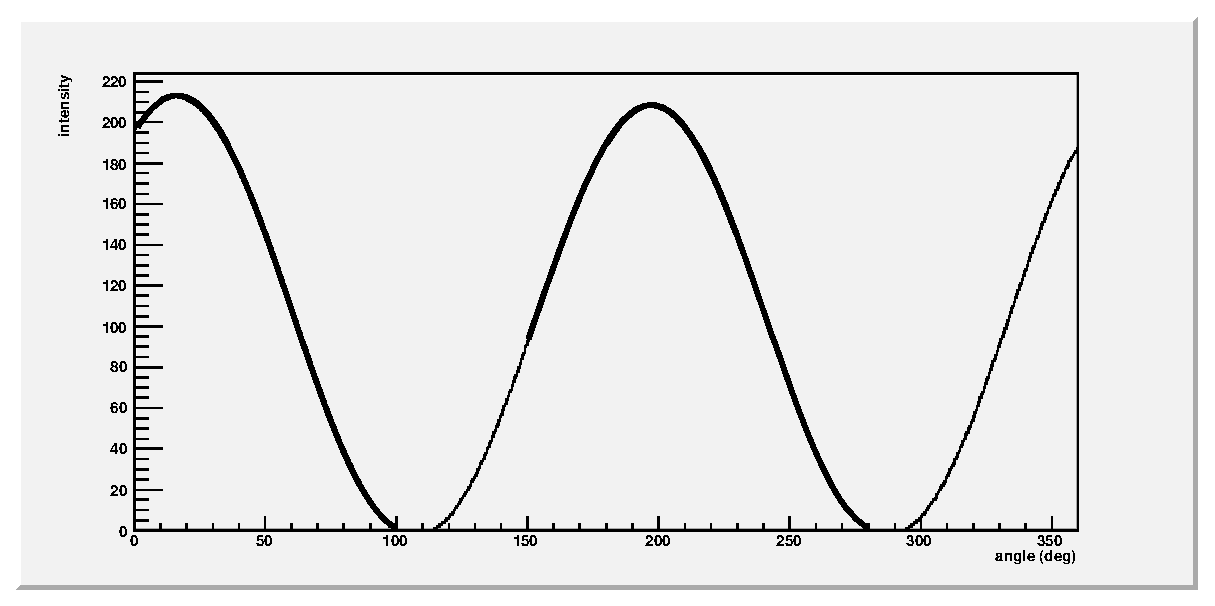
\includegraphics[scale=.6]{3polar.eps}
\caption{Grafico con angolo di rotazione in ascissa e intensità luminosa in ordinata, realizzato con corrente di intensità \unit[3]{A}. Attorno ai due massimi sono visibili le curve prodotte dai fit sinusoidali.}\label{3amp}
\end{figure}
\begin{figure}[!h]\centering
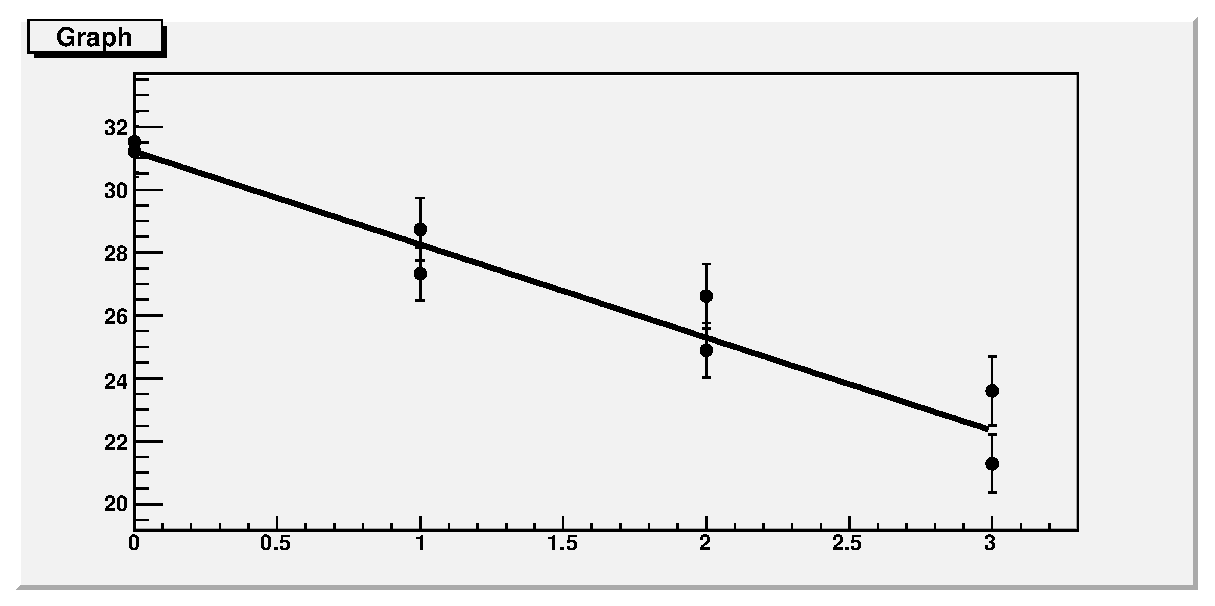
\includegraphics[scale=.6]{graph.eps}
\caption{Grafico con intensità di corrente (\unit{A}) in ascissa e fasi delle curve di intensità della luce in ordinata (\unit{rad}).}\label{lin}
\end{figure}
\end{document}

